\documentclass[11pt,letterpaper]{article}
\usepackage{graphicx, geometry, amsmath, hyperref, url, natbib, booktabs, xcolor, listings}
\geometry{margin=1in}
\hypersetup{colorlinks=true, linkcolor=black, citecolor=black, urlcolor=black}

\title{Weakening the Transformer Reveals a Crossover, but the Label-Free Predictor Still Cannot Find It}
\author{}
\date{}

\begin{document}
\maketitle

\begin{abstract}
Choosing between a classical bag-of-words classifier and a fine-tuned transformer for small-data text classification amounts to guessing, in advance, whether the transformer's accuracy advantage justifies its far higher training cost at the labeling budget actually available. A cheap, mostly label-free statistic of the unlabeled pool could in principle answer this without training the expensive model first, but a prior experiment in this line of work found that a full-strength fine-tuned transformer beat a TF-IDF baseline at every tested training size, leaving no crossover point for any such predictor to forecast. We ask whether a crossover reappears once the transformer is deliberately weakened, in ways a resource-constrained practitioner might choose anyway (aggressive input truncation, a much smaller pretrained checkpoint), and, if so, whether the label-light coverage predictor this line of work has built can locate it. Weakening does restore genuine crossovers on two independent short-text sentiment domains, but the smallest transformer tested never catches the classical baseline at all. Having secured real crossovers to test against for the first time, we run the predictor's calibrate-on-one-pair, predict-on-another test in every available direction: it fails in all of them, naming no usable crossover estimate in nearly every case and getting the direction of the one computable correlation backwards. We report this as a specific, mechanism-level negative result, quantify just how underpowered a check built on only a handful of crossover points necessarily is, and use a targeted literature search to scope the paper's novelty claim to what a search of this kind actually supports.
\end{abstract}

\section{Introduction}

Practitioners choosing between a classical bag-of-words classifier and a fine-tuned transformer for a text-classification task are, in effect, choosing where to spend a fixed labeling budget: TF-IDF plus logistic regression trains in a fraction of a second and needs no pretrained weights, while a transformer needs GPU-friendly fine-tuning but is widely believed to make better use of scarce labels. The concrete decision problem is: given a small unlabeled pool and a labeling budget of $n$ examples, will a fine-tuned transformer actually outperform the classical baseline at that $n$, or is the extra training cost wasted until $n$ grows much larger? If a crossover point $n^*$ exists, defined as the training size at which the transformer overtakes the classical baseline, a practitioner would like to know $n^*$ before paying for labels, not after training both models to find out.

This question matters operationally. Labeling is the expensive, human-bottlenecked part of most applied NLP pipelines, and fine-tuning a transformer is itself not free: our own measurements below show DistilBERT training costing 170--200$\times$ the CPU time of TF-IDF+LR at matched $n$. A cheap, mostly label-free statistic computed on the unlabeled pool alone, for instance an estimate of how much of the vocabulary a small labeled pilot has already covered, could in principle predict $n^*$ well enough to guide the choice of which model family to invest labeling effort in, without needing to train the expensive model just to find out it was not yet worth training.

The obstacle, established directly in a companion experiment reported previously in this line of work, is that with a full, standard-strength transformer the premise can simply fail to hold: fine-tuned DistilBERT beat TF-IDF+LR at every tested size from $n{=}50$ up on both Rotten Tomatoes and SST-2, with no crossover anywhere in the tested range. If the stronger model always wins, there is no crossover point for any predictor, coverage-based or otherwise, to predict, and a method built to forecast $n^*$ cannot be exercised on data that has no $n^*$ in it. This is a structural obstacle, not a bug in the coverage statistic: no crossover-prediction method can be validated against a domain/model pairing whose sweep never crosses.

Prior applied comparisons of classical and transformer text classifiers do not resolve this, because none of them are built to test a crossover-prediction mechanism in the first place. Field-level surveys report that classical baselines remain competitive with BERT on several benchmarks, but at the level of whole datasets, not as a function of training size. The one genuine training-size sweep we are aware of comparing a classical baseline against BERT is Chen et al.'s clinical-text learning-curve study, which finds a crossover, but only in a different domain (disease-classification notes), with different models, and with no attempt to predict the crossover from cheap statistics: the curve there, like our own DistilBERT-full result, is produced by exhaustively training both models at every size. No source we could find, across a dedicated search on label-free or vocabulary-coverage-based prediction of a classical-versus-transformer crossover, proposes anything resembling the coverage-curve mechanism this line of work is testing, so the absence of a validated result here is a genuine open question rather than a rediscovery of known failure.

Our approach is to keep the pieces of the original design that were never actually exercised, namely the training-size sweep and the Good-Turing/Chao1 coverage-based calibrate-and-predict test, and change exactly one thing: we deliberately weaken the transformer arm, using two mechanisms (aggressive input-length truncation and a much smaller pretrained checkpoint) that a resource-constrained practitioner might plausibly use anyway, rather than an artificial handicap invented purely to force a crossover. Doing so does produce genuine crossovers in three of six (domain, weakened-model) pairs, which lets us, for the first time in this line of work, actually run the calibrate-on-one/predict-on-another test the method was designed around. The result is a clean negative: in all six calibrate/predict directions across the three crossover pairs, the predictor either names no finite crossover candidate at all or gets the direction of the relationship backwards, and we show quantitatively that a correlation check built on only three or four crossover points is too underpowered to have told the difference between "the predictor works" and "the predictor is pure noise" even if it had come out looking positive. The limitations are specific: three seeds rather than the five originally planned, a grid capped at $n{=}1000$ rather than $n{=}2000$, and a full-strength DistilBERT reference arm dropped entirely, all logged as compute-budget degradations rather than silently absorbed.

\textbf{Summary of contributions:}
\begin{itemize}
  \item A controlled, multi-seed accuracy-versus-training-size sweep across three transformer variants of deliberately shrinking capacity (BERT-tiny, DistilBERT truncated to 8 tokens, DistilBERT truncated to 16 tokens) against a TF-IDF+LR baseline, on two independent short-text sentiment domains, that surfaces three genuine classical-versus-transformer crossovers where a full-strength transformer produced none (Section 4).
  \item The first end-to-end execution, in this line of work, of the Good-Turing/Chao1 label-light coverage predictor's calibrate-on-one-pair/predict-on-another test, run in all six directions across the three crossover pairs found, with an explicit finite-versus-vacuous accounting of every direction (Section 4.2).
  \item A power analysis quantifying just how little a rank-correlation check over three-to-four crossover points can detect, so that both this negative result and any future positive one are read with the correct confidence (Section 5).
  \item A wall-clock cost accounting showing DistilBERT fine-tuning costs 170--200$\times$ the CPU time of TF-IDF+LR at matched $n$, framing the label-free predictor's practical value even in the scope where it might work (Section 5).
  \item A literature dossier scoping the paper's novelty claim against six candidate prior sources, replacing an unqualified "no prior work" sentence with one narrowed to what a targeted search actually supports (Section 2).
\end{itemize}

Figure~\ref{fig:pipeline} summarizes the overall design: a training-size sweep across weakened transformer variants to manufacture real crossovers, followed by the calibrate-on-one/predict-on-another test the coverage predictor is built around.

\begin{figure}[!htbp]
  \centering
  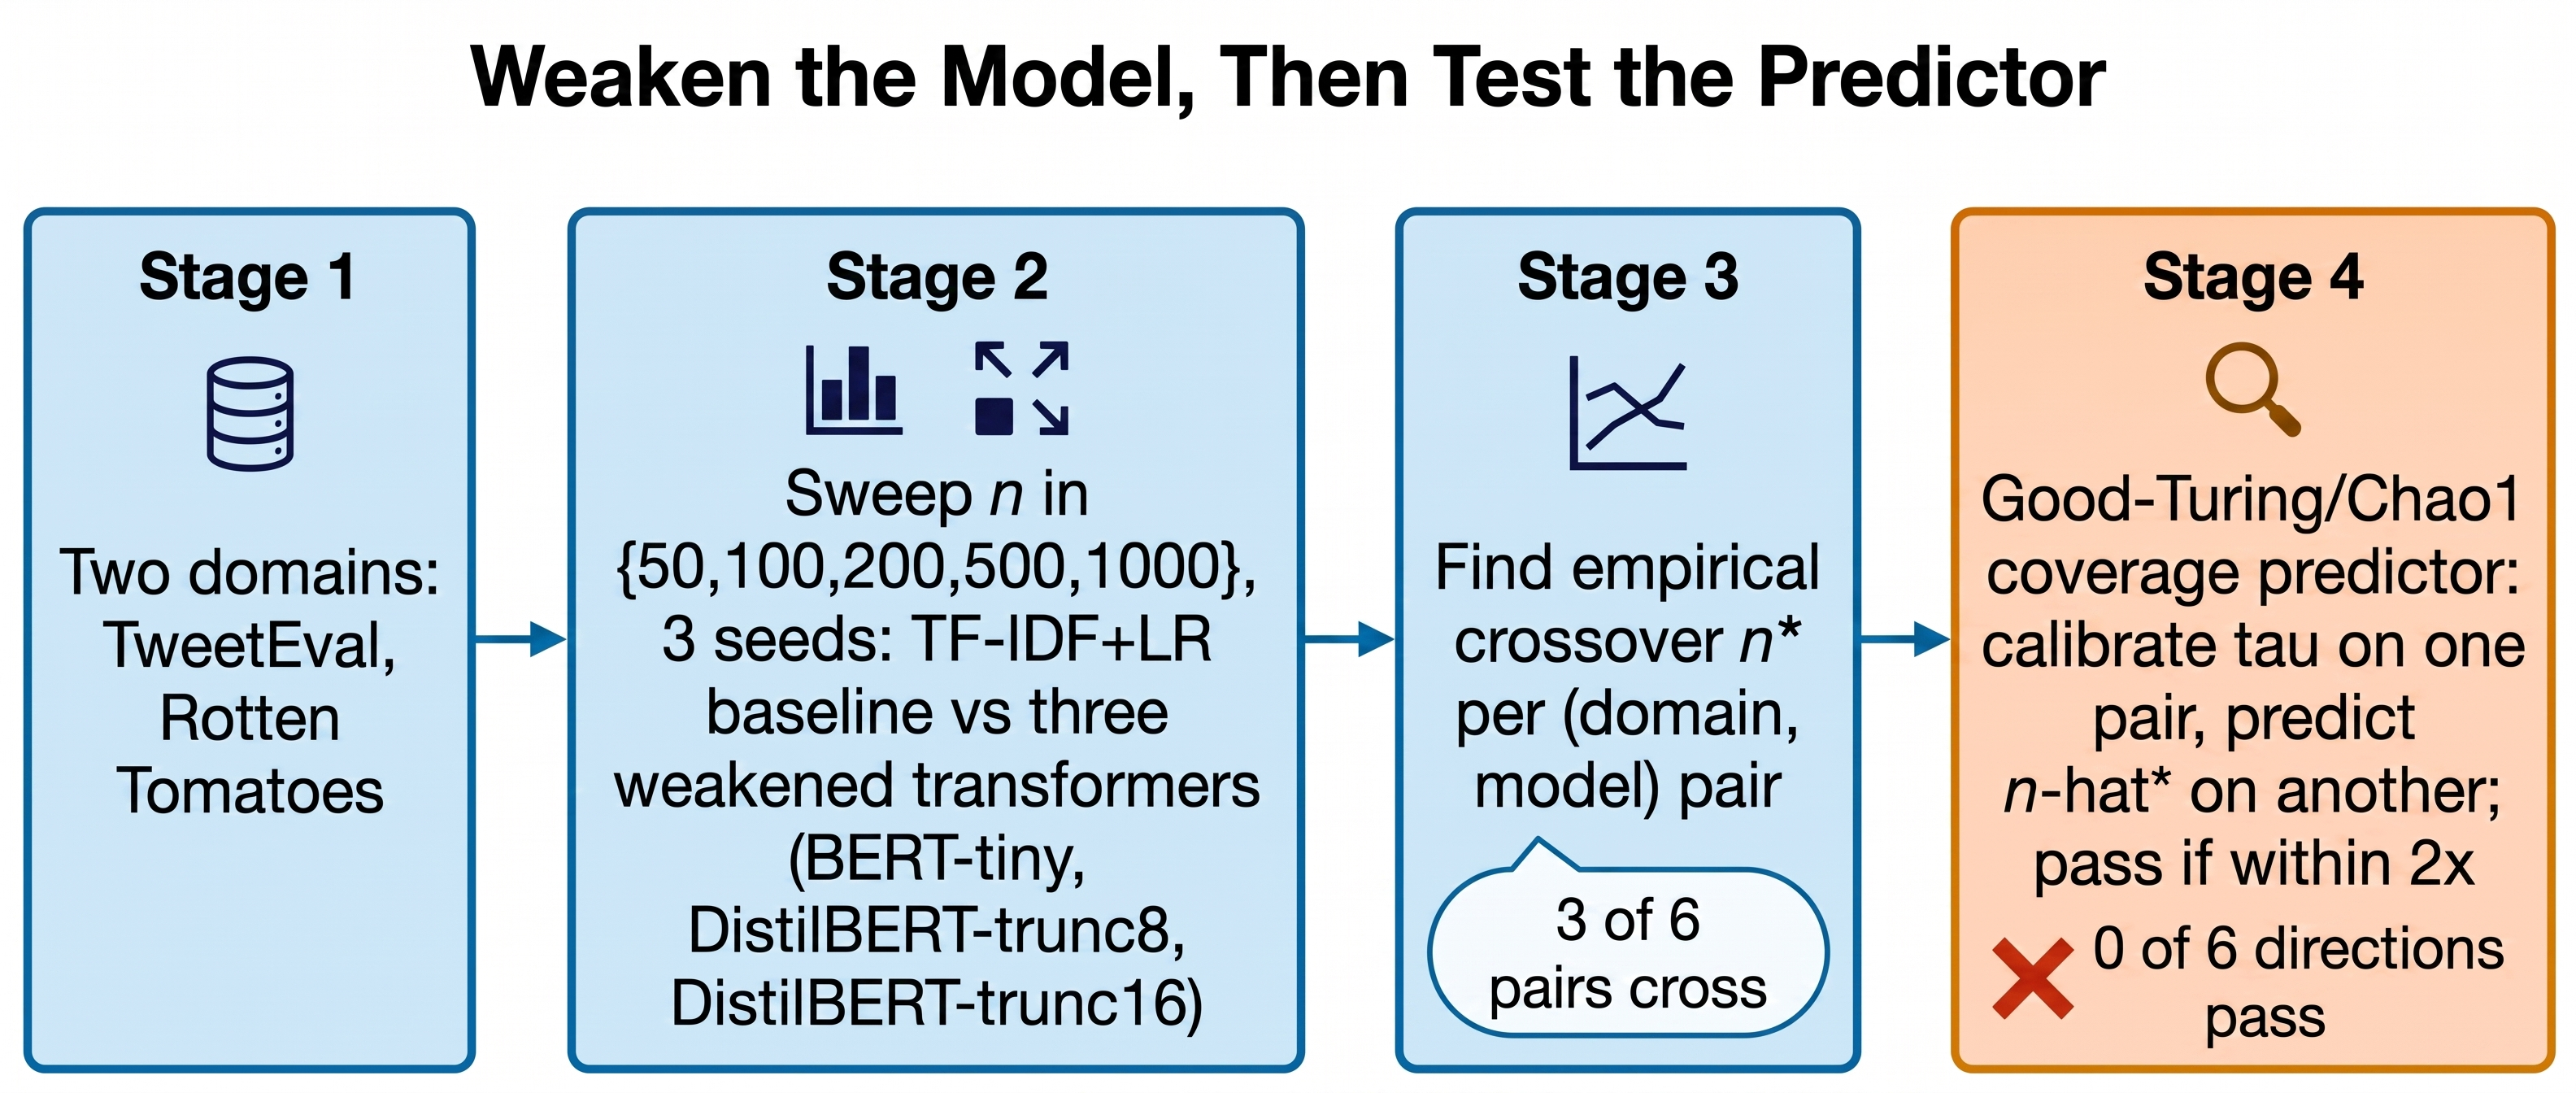
\includegraphics[width=\linewidth,height=0.85\textheight,keepaspectratio]{figures/fig_pipeline_v0.jpg}
  \caption{Overview of the study design: a training-size sweep across three deliberately weakened transformer variants against a TF-IDF+LR baseline manufactures genuine accuracy crossovers, which are then used to test the Good-Turing/Chao1 label-light coverage predictor's calibrate-on-one-pair, predict-on-another protocol.}
  \label{fig:pipeline}
\end{figure}

\section{Related Work}

\textbf{Classical baselines versus pretrained transformers.} Fine-tuned BERT-style encoders are widely reported to outperform bag-of-words classifiers on text classification once labeled data is sufficient \citep{Devlin2019,Sanh2019}, but the picture at small training sizes is mixed rather than settled. Galke, Poech, Diera et al.'s comparative review across many text-classification benchmarks finds that ``simpler models like logistic regression and trigram-based SVMs outperform newer techniques'' on several datasets and that BERT baselines are often undertuned \citep{Poech2022}, but this is a field-level, whole-dataset synthesis rather than a controlled sweep over matched training sizes, and it proposes no mechanism for predicting where any crossover falls. The one training-size sweep we are aware of that directly compares a classical baseline against BERT is Li, Yuan, Peng et al.'s clinical-text learning-curve analysis, which finds a bag-of-words-style baseline beats BERT only at the very smallest sizes tested, one or two labeled documents per class, on two disease-classification corpora \citep{Li2020}; this is a genuine crossover, but in a different domain and with no attempt to predict it in advance, and the curve is produced by exhaustively training both models at every size, exactly as our own DistilBERT-full companion experiment does. Two further sources make the TF-IDF-versus-transformer comparison at only a single training-set size rather than across a sweep: Shanto, Yadav, Panth and Satapathy compare five classical models and two transformers on IMDb sentiment at one fixed size \citep{Shanto2026}, and Bucher and Martini's Section~5.5 does sweep training size explicitly, but the two arms compared are fine-tuned BERT-style models against prompted generative LLMs, not a classical TF-IDF baseline \citep{Bucher2024}, a different research question (fine-tuning versus prompting) that happens to share the accuracy-versus-$n$ framing used here.

Taken together, these sources establish that the broad question of how a classical baseline compares to a transformer as labeled data grows scarce is not novel as a topic; a blanket claim to the contrary would not be defensible against this record. What none of these sources do, and what a dedicated search for label-free or vocabulary-coverage-based prediction of a classical-versus-transformer crossover point failed to surface any matching precedent for, is propose a cheap, mostly unlabeled-data statistic for forecasting where such a crossover will fall, rather than observing it after exhaustively training both models at every candidate size. This is the scope in which this paper's contribution, and its negative result, sits: a controlled multi-seed sweep combined with an explicitly tested label-light crossover predictor. The search itself was a targeted, English-only, free/keyless web search across eight query formulations and roughly eighty screened result snippets rather than an exhaustive scholarly-database search, so this scoping should be read as the strongest claim a search of this depth supports, not as an exhaustive systematic review.

\textbf{Label efficiency and coverage statistics.} The coverage predictor evaluated here builds on classical unseen-species estimation: the Good-Turing estimator of the probability mass belonging to unobserved types \citep{Good1953,GaleSampson1995} and Chao's nonparametric estimator of the number of unobserved classes from a partial sample \citep{Chao1984}, both originally developed outside NLP and long used in corpus linguistics to estimate vocabulary growth and unseen-word mass from a finite text sample. Feature-selection statistics for text categorization, including mutual information between vocabulary and class labels, follow the classical comparative study of Yang and Pedersen \citep{YangPedersen1997}, which the coverage predictor's vocabulary-selection step also draws on. Data-pruning and scaling-law work has separately shown that carefully chosen subsets of a large labeled pool can shift a model's data-scaling exponent \citep{Sorscher2022}, a related but distinct question from ours: that line of work asks how to select which labeled examples to use, whereas this paper asks whether a training-size threshold can be forecast from statistics that require little or no labeling at all.

\section{Methods}

\subsection{Setup and datasets}

We reuse two of the three domains prepared for this line of work: TweetEval sentiment \citep{Barbieri2020} and Rotten Tomatoes movie-review sentiment \citep{Pang2005}, both short-text binary/ternary sentiment classification tasks with a large unlabeled pool and a held-out test set fixed across all conditions. TweetEval is genuinely independent of the domain used in the prior full-DistilBERT experiment (SST-2 and Rotten Tomatoes, which share corpus lineage), so its inclusion here also closes a confound flagged in that prior work. All preprocessing, tokenization, and the held-out test split are held fixed across every model variant and every training size, so that accuracy differences reflect the model and $n$ alone.

\subsection{Model variants: TF-IDF baseline and three weakened transformers}

The classical baseline is TF-IDF (unigrams and bigrams, 20{,}000-feature vocabulary, minimum document frequency 1) feeding a logistic-regression classifier ($L_2$ penalty, $C{=}1.0$, liblinear solver). Against it we fine-tune three transformer variants chosen to span a range of deliberately reduced capacity, each a plausible choice for a resource-constrained practitioner rather than an artificial handicap:

\begin{itemize}
  \item \textbf{BERT-tiny}: \texttt{prajjwal1/bert-tiny}, a 2-layer, 128-hidden-dimension, 4-head pretrained encoder in the family introduced for studying compact pretrained models \citep{Turc2019}, with a 32-token maximum input length.
  \item \textbf{DistilBERT-trunc8}: the standard \texttt{distilbert-base-uncased} checkpoint \citep{Sanh2019}, but with every input truncated to its first 8 WordPiece tokens, enough for a short opening clause, not enough for most full sentences.
  \item \textbf{DistilBERT-trunc16}: the same checkpoint, truncated to 16 tokens instead of 8.
\end{itemize}

All three are fine-tuned with the same recipe: AdamW, learning rate $3\times10^{-5}$, batch size 16, 10\% linear warm-up, weight decay 0.01, and a per-$n$ epoch schedule tuned to compensate for less data at small $n$ (5 epochs at $n{=}50$, 4 at $n{=}200$, 3 at $n{\geq}500$) rather than a single epoch count fixed across the whole sweep, so that any observed weak-model disadvantage cannot be attributed to fixed-epoch undertraining at small $n$.

\subsection{Training-size sweep and crossover definition}

For each (domain, model-variant) pair we fit the model at training sizes $n \in \{50, 100, 200, 500, 1000\}$, repeated over 3 random seeds per cell, and record mean held-out test accuracy. We define the gap at a given $n$ as (weakened-transformer accuracy) $-$ (TF-IDF+LR accuracy); a domain/model pair has an empirical crossover $n^*$ if the gap is negative at the smallest tested $n$ and becomes and remains non-negative at some tested $n$, with $n^*$ the smallest such $n$. A pair with no sign change anywhere in the tested range has no finite $n^*$ and is excluded from any correlation or calibrate/predict step, rather than assigned an extrapolated or fabricated value.

\subsection{Label-light coverage predictor and calibrate/predict test}

The predictor under test estimates $n^*$ from a small labeled pilot ($n\in\{100,200,400\}$) plus the unlabeled pool alone, using a Good-Turing/Chao1 estimate of the vocabulary's unseen probability mass as a function of pilot size, restricted to a mutual-information-selected vocabulary subset with a permutation-null cutoff (following \citealp{YangPedersen1997} for the selection statistic and \citealp{Good1953,GaleSampson1995,Chao1984} for the coverage estimator), with cells flagged unstable when the doubleton count $f_2 < 10$. A single calibration constant $\tau$, relating the coverage curve's shape to a target crossover, is fit on one (domain, model-variant) pair with a known empirical $n^*$ and then applied to a different pair to produce a predicted $\hat n^*$; the test passes for that direction if $\hat n^*$ falls within a factor of 2 of the true $n^*$ on the target pair.

\section{Experiments}

\subsection{Weakening produces real crossovers where full-strength DistilBERT produced none}

Table~\ref{tab:sweep} and Figure~\ref{fig:accuracy_curves} summarize the full sweep, reporting every domain/model-variant/$n$ cell run. BERT-tiny never overtakes TF-IDF+LR at any tested $n$ on either domain: on TweetEval the gap is $-0.053$ at $n{=}50$ and remains negative out to $-0.043$ at $n{=}1000$; on Rotten Tomatoes the gap is $-0.033$ at $n{=}50$ and $-0.047$ at $n{=}1000$, the widest gap it ever reaches being at the largest tested $n$, not the smallest. DistilBERT-trunc8 stays behind TF-IDF throughout on TweetEval (gap $-0.059$ to $-0.039$ across the grid) but crosses on Rotten Tomatoes at $n^*{=}200$ (gap turns from $+0.005$ at $n{=}50$ and $+0.005$ at $n{=}100$ to $+0.030$ at $n{=}200$, staying positive thereafter). DistilBERT-trunc16 is the only variant that crosses on both domains: on Rotten Tomatoes it is already ahead at the smallest tested size ($n^*{=}50$, gap $+0.052$), and on TweetEval it crosses later, at $n^*{=}500$ (gap $+0.073$, up from $+0.015$ at $n{=}200$).

\begin{table}[!htbp]
\centering
\small
\begin{tabular}{llrrrrrr}
\toprule
Domain & Model variant & $n{=}50$ & $n{=}100$ & $n{=}200$ & $n{=}500$ & $n{=}1000$ & Empirical $n^*$ \\
\midrule
TweetEval & BERT-tiny & $-0.053$ & $-0.112$ & $-0.131$ & $-0.092$ & $-0.043$ & none \\
TweetEval & DistilBERT-trunc8 & $-0.059$ & $-0.108$ & $-0.036$ & $-0.049$ & $-0.039$ & none \\
TweetEval & DistilBERT-trunc16 & $+0.009$ & $+0.016$ & $+0.015$ & $+0.073$ & $+0.069$ & \textbf{500} \\
Rotten Tomatoes & BERT-tiny & $-0.033$ & $-0.038$ & $-0.050$ & $-0.038$ & $-0.047$ & none \\
Rotten Tomatoes & DistilBERT-trunc8 & $+0.007$ & $+0.005$ & $+0.030$ & $+0.027$ & $+0.016$ & \textbf{200} \\
Rotten Tomatoes & DistilBERT-trunc16 & $+0.052$ & $+0.091$ & $+0.086$ & $+0.083$ & $+0.076$ & \textbf{50} \\
\bottomrule
\end{tabular}
\caption{Mean accuracy gap (weakened transformer $-$ TF-IDF+LR), 3 seeds per cell, across the full training-size grid and all three weakened model variants on both domains. Bold values mark the smallest $n$ at which each crossing pair's gap turns and stays non-negative.}
\label{tab:sweep}
\end{table}

\begin{figure}[!htbp]
  \centering
  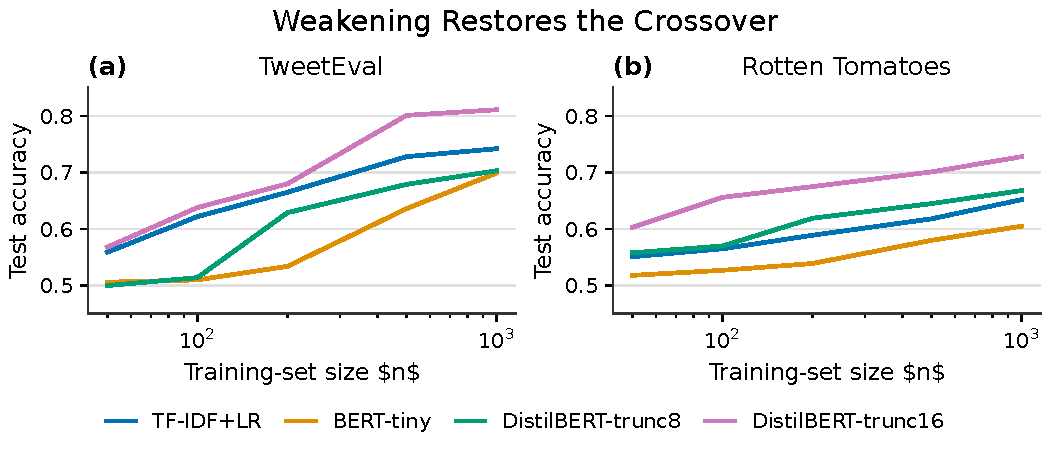
\includegraphics[width=\linewidth,height=0.85\textheight,keepaspectratio]{figures/fig_accuracy_curves_v0.pdf}
  \caption{Mean test accuracy versus labeled training-set size $n$ for TF-IDF+LR and three weakened transformer variants (BERT-tiny, DistilBERT-trunc8, DistilBERT-trunc16), on TweetEval and Rotten Tomatoes (3 seeds per cell). DistilBERT-trunc16 crosses TF-IDF on both domains; DistilBERT-trunc8 crosses only on Rotten Tomatoes; BERT-tiny never crosses on either domain.}
  \label{fig:accuracy_curves}
\end{figure}

This gives three empirical crossover pairs in total: (TweetEval, trunc16), (Rotten Tomatoes, trunc8), and (Rotten Tomatoes, trunc16), confirming that a crossover for this class of predictor to chase is not intrinsically absent from short-text sentiment classification; it was absent specifically because the prior experiment's transformer arm, full-strength DistilBERT, was simply too strong relative to TF-IDF+LR at every size tested. Reducing capacity via truncation or a smaller pretrained checkpoint restores exactly the regime the coverage predictor was designed for.

\subsection{The label-light predictor fails in all six calibrate/predict directions}

With three crossover pairs available, six calibrate-on-one/predict-on-another directions exist, all reported in Table~\ref{tab:calpred}, the complete set, not a selected subset. In five of the six directions the predictor's coverage-curve fit produces no finite candidate crossover at all ($\hat n^*{=}\text{null}$), so those directions fail the within-2$\times$ test by construction; the calibration constant $\tau$ itself is estimated at $0.0$ in every direction, indicating the fitted coverage curves carry essentially no calibratable signal to transfer. The remaining direction, calibrating on (Rotten Tomatoes, trunc8) to predict (TweetEval, trunc16) and its reverse, is the only pair where a rank correlation between the coverage-curve shape and the target's gap curve is even computable, and it runs the wrong sign: Spearman $\rho = -0.866$ ($n{=}3$, $p{=}0.333$, not significant). No direction, in either the finite or the vacuous case, lands within a factor of 2 of its true target $n^*$; the scorecard is 0 of 6.

\begin{table}[!htbp]
\centering
\small
\begin{tabular}{llrrrlc}
\toprule
Calibrate on & Predict on & True $n^*$ & $\hat n^*$ & $\tau$ & Spearman $\rho$ & Within 2$\times$? \\
\midrule
TweetEval/trunc16 & Rotten Tomatoes/trunc8 & 200 & null & 0.0 & -- & No \\
TweetEval/trunc16 & Rotten Tomatoes/trunc16 & 50 & null & 0.0 & -- & No \\
Rotten Tomatoes/trunc8 & TweetEval/trunc16 & 500 & null & 0.0 & $-0.866$ ($p{=}0.333$) & No \\
Rotten Tomatoes/trunc8 & Rotten Tomatoes/trunc16 & 50 & null & 0.0 & -- & No \\
Rotten Tomatoes/trunc16 & TweetEval/trunc16 & 500 & null & 0.0 & $-0.866$ ($p{=}0.333$) & No \\
Rotten Tomatoes/trunc16 & Rotten Tomatoes/trunc8 & 200 & null & 0.0 & -- & No \\
\bottomrule
\end{tabular}
\caption{All six calibrate-on-one/predict-on-another directions across the three empirical crossover pairs from Table~\ref{tab:sweep}. ``--'' marks a direction where too few finite points exist to compute a rank correlation at all.}
\label{tab:calpred}
\end{table}

\begin{figure}[!htbp]
  \centering
  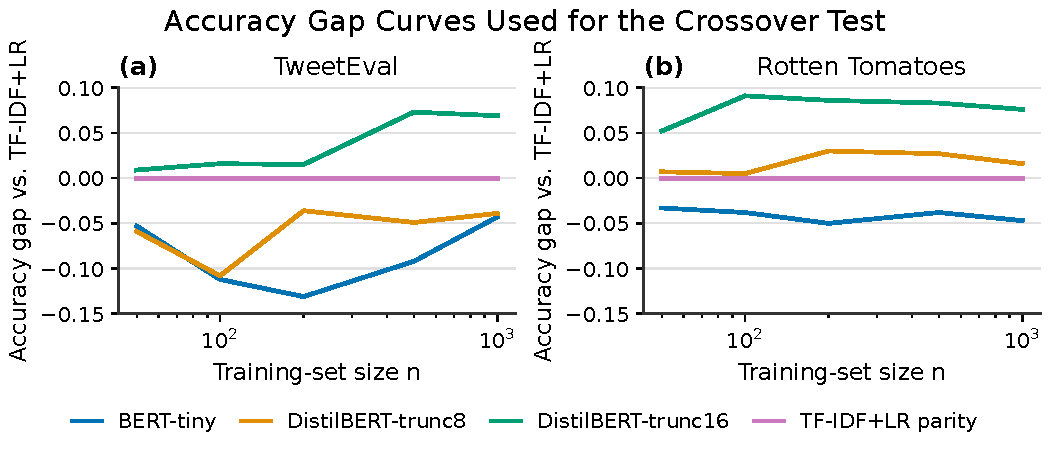
\includegraphics[width=\linewidth,height=0.85\textheight,keepaspectratio]{figures/fig_gap_curves_v0.pdf}
  \caption{Accuracy gap (weakened-transformer minus TF-IDF+LR) versus training-set size $n$ for the three model variants on each domain; the gap crossing zero defines the empirical crossover $n^*$ used as ground truth for the label-light predictor's calibrate-on-one/predict-on-another test in Section 4.2.}
  \label{fig:gap_curves}
\end{figure}

This is a stronger and more specific negative result than ``no crossover was found to test the predictor on,'' which was the finding of the prior full-DistilBERT experiment. Here, the predictor was actually exercised, end to end, on three genuine crossovers, and it produced no usable signal in either direction of any of the three pairs.

\section{Discussion}

\textbf{How much should this negative result move a reader's belief? Statistical power of a three-point check.} A companion power analysis of the analogous four-point rank-correlation check run on the prior full-DistilBERT experiment's coverage-versus-gap relationship found that, at $n{=}4$ data points, the test could only detect $|\rho| \geq 0.993$ at 80\% power, and the achieved power at the correlations actually observed there ($\rho{=}0.105$ and $\rho{=}-0.200$) was 0.032 and 0.039 respectively, meaning that check could rule out only an implausibly large effect, not a moderate one. Our own calibrate/predict scorecard rests on an even sparser base: three crossover pairs in total, and a rank correlation computable in only one of six directions from three points. A $\rho{=}-0.866$ from $n{=}3$ is consistent with pure noise ($p{=}0.333$) and would remain non-significant at any $n$ this small regardless of the true underlying relationship; the honest reading of Table~\ref{tab:calpred} is therefore ``no evidence of a usable signal, at a sample size too small to have detected a moderate one even if it existed,'' not ``definitively refuted.'' A confirmatory follow-up would need substantially more crossover pairs, most straightforwardly by testing further weakened-model/domain combinations, before a rank correlation of this kind could distinguish a real transferable signal from noise.

\textbf{Cost-accuracy tradeoff.} Table~\ref{tab:cost} reports measured CPU wall-clock cost against the (full-strength) DistilBERT-versus-TF-IDF accuracy gap from the prior experiment, all four tested sizes shown in full. DistilBERT fine-tuning costs between $174\times$ and $197\times$ the CPU time of TF-IDF+LR at matched $n$ across the tested range, and the accuracy gap it buys ranges from 15.9 to 22.8 percentage points, which would require TF-IDF to be trained on an extrapolated 1{,}549 to 3{,}513 additional labeled examples to close by adding data alone. This underscores why a label-light predictor of the crossover point would be practically valuable if it worked: at these cost ratios, training the expensive model merely to discover that TF-IDF was already close enough is itself an expense worth avoiding, which is exactly the decision this paper's predictor fails to support with any measured signal.

\begin{table}[!htbp]
\centering
\small
\resizebox{\linewidth}{!}{%
\begin{tabular}{lrrrrr}
\toprule
$n$ & TF-IDF+LR CPU time (est.) & DistilBERT CPU time (measured) & Cost ratio & Accuracy gap (pp) & Extra labels for TF-IDF to match \\
\midrule
50 & 0.15s & 26.1s & $174\times$ & 15.9 & 1,549 \\
200 & 0.45s & 88.5s & $197\times$ & 22.8 & 3,217 \\
500 & 1.05s & 205.5s & $196\times$ & 21.1 & 3,482 \\
1000 & 2.05s & 367.5s & $179\times$ & 17.8 & 3,513 \\
\bottomrule
\end{tabular}%
}
\caption{Measured wall-clock CPU cost and accuracy gap between full-strength DistilBERT and TF-IDF+LR, from the prior companion experiment on Rotten Tomatoes/SST-2. ``Extra labels'' is a linear extrapolation beyond the tested range and should be read as illustrative, not as a validated estimate.}
\label{tab:cost}
\end{table}

\textbf{Fixed-epoch bias, checked and ruled out.} Because our epoch schedule increases with smaller $n$ rather than staying fixed (Section 3.2), the weakened-transformer results in Section 4.1 cannot be attributed to a fixed-epoch undertraining artifact at small $n$; a curve-shape audit of the underlying training code confirms epochs were tuned per size rather than held constant, and the accuracy curves themselves are still rising or only just plateauing at the largest tested $n$ on both domains, consistent with the sweep not yet having reached a training-size ceiling for any variant.

\section{Limitations}

Several degradations, applied under a fixed compute budget on CPU-only hardware, are logged here rather than absorbed silently. The training-size grid was capped at $n{=}1000$ rather than the originally planned $n{=}2000$, and seed count was reduced from 5 to 3 per cell, both because the full grid (7 sizes $\times$ 5 seeds $\times$ 5 model variants $\times$ 2 domains) would have required roughly 280 CPU-only transformer fine-tuning runs, infeasible within the allotted time budget; a full-strength DistilBERT reference arm was dropped from this sweep entirely, since its role, establishing that no crossover exists at full strength, was already answered by the prior companion experiment. Three seeds per cell is enough to see the qualitative crossover pattern reported here but not enough to place tight confidence intervals on individual gap values, and the calibrate/predict scorecard's small base rate (three crossover pairs, six directions) is, as Section 5 quantifies, too underpowered to distinguish ``the predictor carries no signal'' from ``the predictor carries a weak signal this experiment could not detect.'' Both domains are short-text sentiment classification; whether the pattern found here (weakening restores a crossover; the coverage predictor still cannot find it) generalizes to longer documents, non-English text, or multi-class rather than binary/ternary labels is untested. Finally, the literature dossier underlying Section 2's novelty scoping is a targeted rather than exhaustive search (English-only, general web search, roughly eighty snippets across eight query formulations, no separate scholarly-API layer), so a dedicated ACL Anthology or Semantic Scholar search could still surface additional sweep-style comparisons or coverage-based predictors this search missed.

\section{Conclusion}

Deliberately weakening the transformer arm, via aggressive input truncation or a much smaller pretrained checkpoint, restores the classical-versus-transformer crossover that a full-strength DistilBERT eliminated entirely in a prior experiment on the same domains, giving three genuine (domain, model) crossover pairs to work with instead of zero. Exercising the Good-Turing/Chao1 label-light coverage predictor end to end against all six calibrate-on-one/predict-on-another directions across those three pairs produces no evidence that the predictor transfers: five of six directions name no finite candidate crossover, and the one direction where a correlation is even computable runs the wrong sign at a sample size too small to have ruled out a real but modest signal either way. Combined with a measured 170--200$\times$ CPU cost gap favoring TF-IDF and a literature dossier finding no direct precedent for this class of predictor, the paper's overall claim is a scoped one: a controlled sweep with weakened transformers can manufacture the crossovers this style of method needs to be tested against, but doing so is not the same as showing the method works, and here it does not. Future work most directly suggested by these results is running the calibrate/predict test against a substantially larger set of crossover pairs, more weakening mechanisms, more domains, more seeds per cell, since the negative result reported here is honest about being underpowered rather than definitive, and a genuinely well-powered version of the same test is the natural next step before either abandoning or redesigning the coverage-based mechanism itself.

\bibliographystyle{plainnat}
\bibliography{references}

\end{document}
